\chapter{Loss functions} \label{loss functions}
In order to train the model with different settings, we tried many loss functions. This chapter will show all the loss functions used. The loss functions will be slightly different depending on the process, namely for the training and evaluation phases. There are a total of eight loss functions and their combined loss functions.

\section{MSE loss} \label{mse loss}
% show the MSE \& weighted MSE
\gls{mse} is a common loss function in machine learning. Its formula is written as
\begin{equation}
    \centering
    \mathcal{L}_{\text{MSE}} = \frac{1}{n} \sum_{i=1}^{n} (Y_i - \hat{Y}_i)^2,
\end{equation}

where $Y_i$ represents the ground truth, $\hat{Y}_i$ denotes the prediction and $n$ is the total number of the samples. $\mathcal{L}_{\text{MSE}}$ represents the \gls{mse} loss between the ground truth and prediction, and the goal of the model is to reduce this value. 

But in specific cases, the meaning of $Y_i$ and $\hat{Y}_i$ and the usage of this loss function will be different, that is, the format of the values in ground truth and prediction is depending on the processing methods, namely the red part shown in Figure \ref{postprocessing_block}. Furthermore, it can be formulated into two loss functions according to the needs in the range-Doppler map upsampling task, namely \gls{mse} and \gls{wmse}.

\subsection{MSE} \label{mse subsection}
In normal \gls{mse}, no additional weights are added to the loss function, but it is still performed depending on the different processes, training or evaluation phase.

\begin{spacing}{1.5}
\textbf{\large{Training\&validation phases}}
\end{spacing}
In the phase of training and validation, the meaning of the $Y_i$ and $\hat{Y}_i$ is firstly up to the input data representation, that is, in the case of real and imaginary representation type, the loss of both real and imaginary parts will be calculated separately, where $Y_i$ refers to them of the high-resolution data and $\hat{Y}_i$ denotes that of the super-resolution data accordingly, then both will be combined in the way of
\begin{equation}
    \centering
    \mathcal{L}_{\text{MSE}} = \mathcal{L}_{\text{MSE, Re}} + \mathcal{L}_{\text{MSE, Im}},
\end{equation}

whereas in the case of amplitude and phase representation type, the loss of amplitude and phase will be calculated respectively and combined as
\begin{equation}
    \centering
    \mathcal{L}_{\text{MSE}} = \mathcal{L}_{\text{MSE, Amp}} + \lambda \times \mathcal{L}_{\text{MSE, Ph}},
\end{equation}

where $\lambda$ as a hyperparameter can be tuned according to the processing methods. But if only amplitude, then the phase \gls{mse} loss will be neglected.

\begin{spacing}{1.5}
\textbf{\large{Evaluation phases}}
\end{spacing}
Since a lot of settings and combinations exist, in order to make the evaluation fair for all the cases and due to the importance of the amplitude in the range-Doppler map upsampling, only the amplitude loss will be taken into consideration, that is,
\begin{equation}
    \centering
    \mathcal{L}_{\text{MSE, Amp}} = \frac{1}{n} \sum_{i=1}^{n} (A_i - \hat{A}_i)^2,
\end{equation}

where $A$ and $\hat{A}$ are the amplitude of the high-resolution and super-resolution data, respectively. Note that in the training phase, the training loss is calculated between ground truth $Y$ and prediction $\hat{Y}$ which are before the postprocessing block as shown in Figure \ref{postprocessing_block}. However, in the evaluation phase, the amplitude of the ground truth $A$ and prediction $\hat{A}$ are converted back after the postprocessing block.

\subsection{WMSE}
The large dynamic range of radar signal amplitudes  causes relatively low MSE loss for weak signal parts in comparison to strong reflections. The model will not pay much attention on these signals. Therefore, we assign different weights according to the amplitude of the signal. In order to make the weaker signal also get enough attention and the weaker signals get a larger weight, and the formula of amplitude \gls{wmse} loss will become
\begin{equation}
    \centering
    \mathcal{L}_{\text{WMSE, Amp}} = \frac{1}{n} \sum_{i=1}^{n} \frac{(A_i - \hat{A}_i)^2}{A_i},
    \label{amplitude wmse loss equation}
\end{equation}

while the angle loss in \gls{wmse} is still same as in the \gls{mse} and combine them with an additional weight $\lambda$ as well in the case of the amplitude and phase representation type, namely
\begin{equation}
    \centering
    \mathcal{L}_{\text{WMSE}} = \mathcal{L}_{\text{WMSE, Amp}} + \lambda \times \mathcal{L}_{\text{MSE, Ph}},
\end{equation}

while in the evaluation process, only the amplitude loss part, namely formula \ref{amplitude wmse loss equation}, is used. The reason is same as the explanation in the section \ref{mse subsection}.

\section{SDR loss} \label{sdr loss}
% show the SDR \& SD-SDR
In the field of signal processing, a very important indicator is \gls{snr}. We hope to get a larger signal related to the noise. According to the paper \cite{roux_sdr_2018} by Jonathan et al., the classical \gls{snr} is equivalent to the \texttt{bss\_eval\_images}’s SDR in the case that there's only noise between the ground truth $A$ and prediction $\hat{A}$, that is, 
\begin{equation}
    \centering
    \mathcal{L}_{\text{SDR}} = 10 \log_{10} \left( \frac{\|A\|^2}{\|A - \hat{A}\|^2} \right).
    \label{sdr equation}
\end{equation}

As shown in Figure \ref{illustration of the snr and si-sdr}, Jonathan et al. proposed two loss functions as the variations of the \gls{sdr}, called \gls{si-sdr} and \gls{sd-sdr}, which are respectively written as
\begin{equation}
    \centering
    \mathcal{L}_{\text{SI-SDR}} = 10 \log_{10} \left( \frac{\| e_{\text{target}} \|^2}{\| e_{\text{res}} \|^2} \right) = 10 \log_{10} \left(\frac{\left\| \frac{\hat{Y}^{T} Y}{\|Y\|^2} Y \right\|^2}{\left\| \frac{\hat{Y}^{T} Y}{\|Y\|^2} Y - \hat{Y} \right\|^2}\right),
\end{equation}

\begin{equation}
    \centering
    \mathcal{L}_{\text{SD-SDR}} = 10 \log_{10} \left( \frac{\|\alpha s\|^2}{\|s - \hat{s}\|^2} \right) = \mathcal{L}_{\text{SDR}} + 10 \log_{10} \alpha^2,
\end{equation}

where the optimal scaling factor is $\alpha = \hat{Y}^{T} Y / \|Y\|^2$. The advantage of these two variations is the faster convergence, but the \gls{si-sdr} is sensitive to the scaling and \gls{sd-sdr} is not sure in the frequency domain. Therefore, we keep using the classical \gls{sdr} loss, namely formula \ref{sdr equation}. Moreover, the current \gls{sdr} is better when it's larger, so to make it decrease during the training process, a negative sign is added.

\begin{figure}
	\centering
	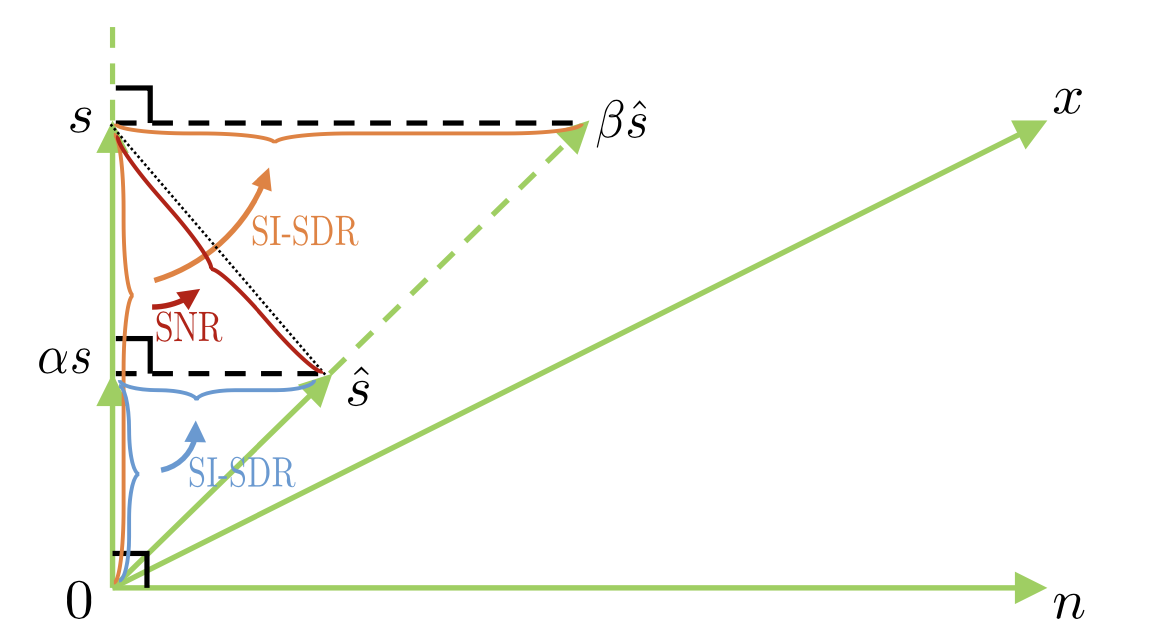
\includegraphics[scale=.55]{thesis/figures/sdr.png}
	\caption{Illustration of the SNR and SI-SDR \cite{roux_sdr_2018}}
	\label{illustration of the snr and si-sdr}
\end{figure}

\section{LSD loss} \label{lsd loss}
% show the LSD and PLSD
Braun et al. proposed two loss functions \cite{braun_consolidated_2020}, \gls{lsd} and \gls{plsd}, which add logarithmic operation on the amplitude compared to classical \gls{mse} and are beneficial for the range-Doppler maps with the significant amplitude fluctuation.

\subsection{LSD}
\gls{lsd} can be described as
\begin{equation}
    \centering
    \mathcal{L}_{\text{LSD, Amp}} = \left\langle \left| \log_{10} \hat{A} - \log_{10} A \right|^2 \right\rangle,
\end{equation}

where $A$ represents the amplitude of each point in the range-Doppler map and
\begin{equation}
    \centering
    \left\langle P(h, w) \right\rangle = \frac{1}{H W} \sum_{h,w} P(h, w).
\end{equation}

To improve the stability further, the root mean square operation can combine with the \gls{lsd} loss function, it turns to
\begin{equation}
    \centering
    \mathcal{L}_{\text{LSD, Amp}} = \left\{ \frac{1}{N} \sum_{n=1}^{N} \left[ \log_{10} A(n) - \log_{10} \hat{A}(n) \right]^p \right\}^{\frac{1}{p}},
    \label{final lsd equation}
\end{equation}

where $p$ is set as 2. With the use of logarithmic operations, the amplitude change will be obviously reduced. However, since the data with high amplitude in the range-Doppler map is relatively only a small part while the part in the longer range or velocity in range-Doppler map occupy the majority, the model will pay much attention on the background noise during the training process, affecting the final super-resolution range-Doppler map. Therefore, a mask is added on the \gls{lsd} loss to ignore much background noise during the training process. The threshold is set according to the median value or the percentile, only the loss of the part which has the amplitude over the threshold will be taken into consideration, otherwise will be neglected. The mask is still based on the logarithm amplitude. If the percentile is set as 50\%, i.e. 50\% data can over the threshold, the mask looks like Figure \ref{mask in the percentile of 70}, where Figure \ref{high resolution image with logarithic amplitude} shows the corresponding high-resolution range-Doppler map with the logarithmic amplitude and Figure \ref{masked high resolution image with logarithic amplitude} illustrates the masked high-resolution range-Doppler map.

\begin{figure}
    \centering
    \hspace{-0.6cm}
    \begin{subfigure}{0.32\textwidth}
        \centering
        \adjustbox{height=3cm}{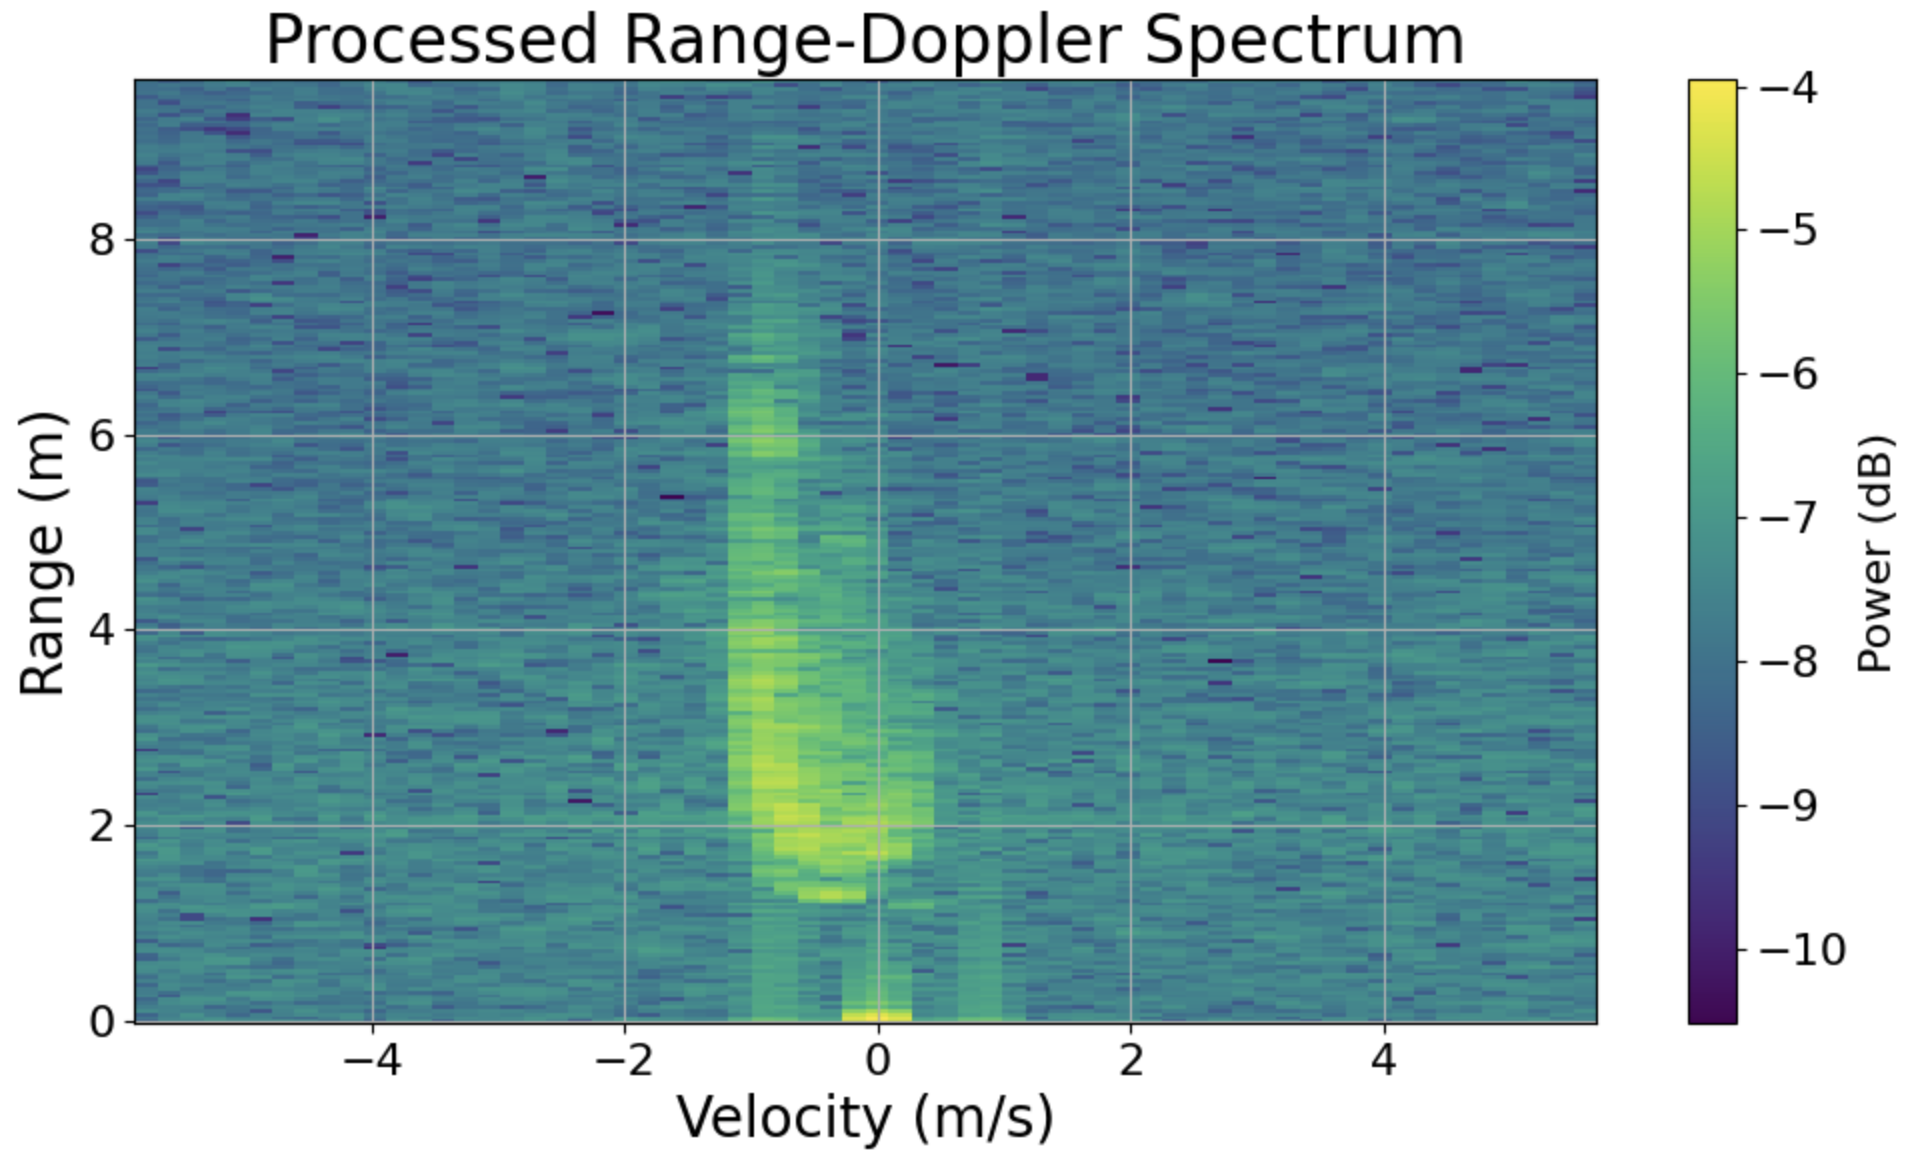
\includegraphics[scale=.24]{thesis/figures/gt_logamp.png}}
        \caption{Processed high-resolution range-Doppler map}
        \label{high resolution image with logarithic amplitude}
    \end{subfigure}
    \begin{subfigure}{0.32\textwidth}
        \centering
        \adjustbox{height=3cm}{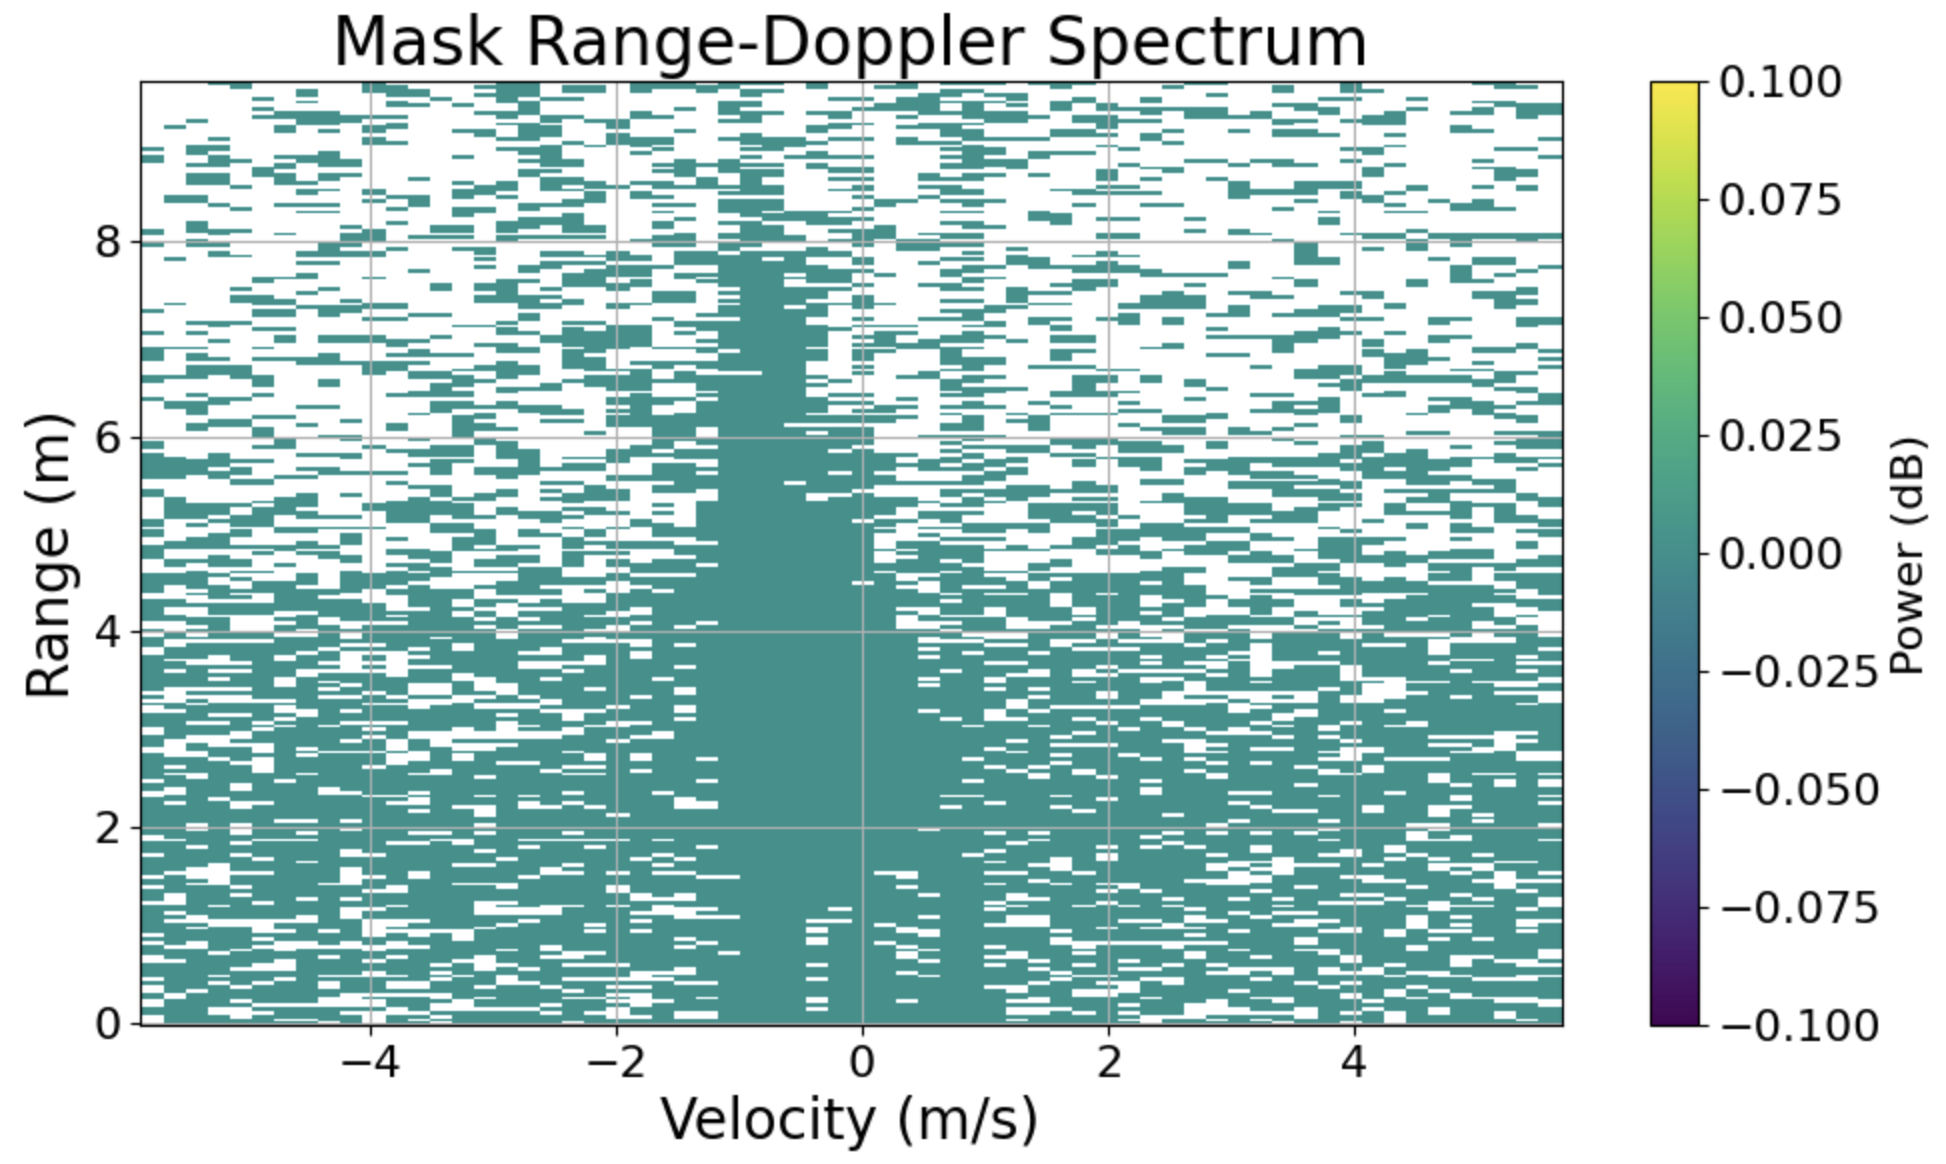
\includegraphics[scale=.24]{thesis/figures/mask.png}}
        \caption{The mask in the percentile of 50\%}
        \label{mask in the percentile of 70}
    \end{subfigure}
    \begin{subfigure}{0.32\textwidth}
        \centering
        \adjustbox{height=3cm}{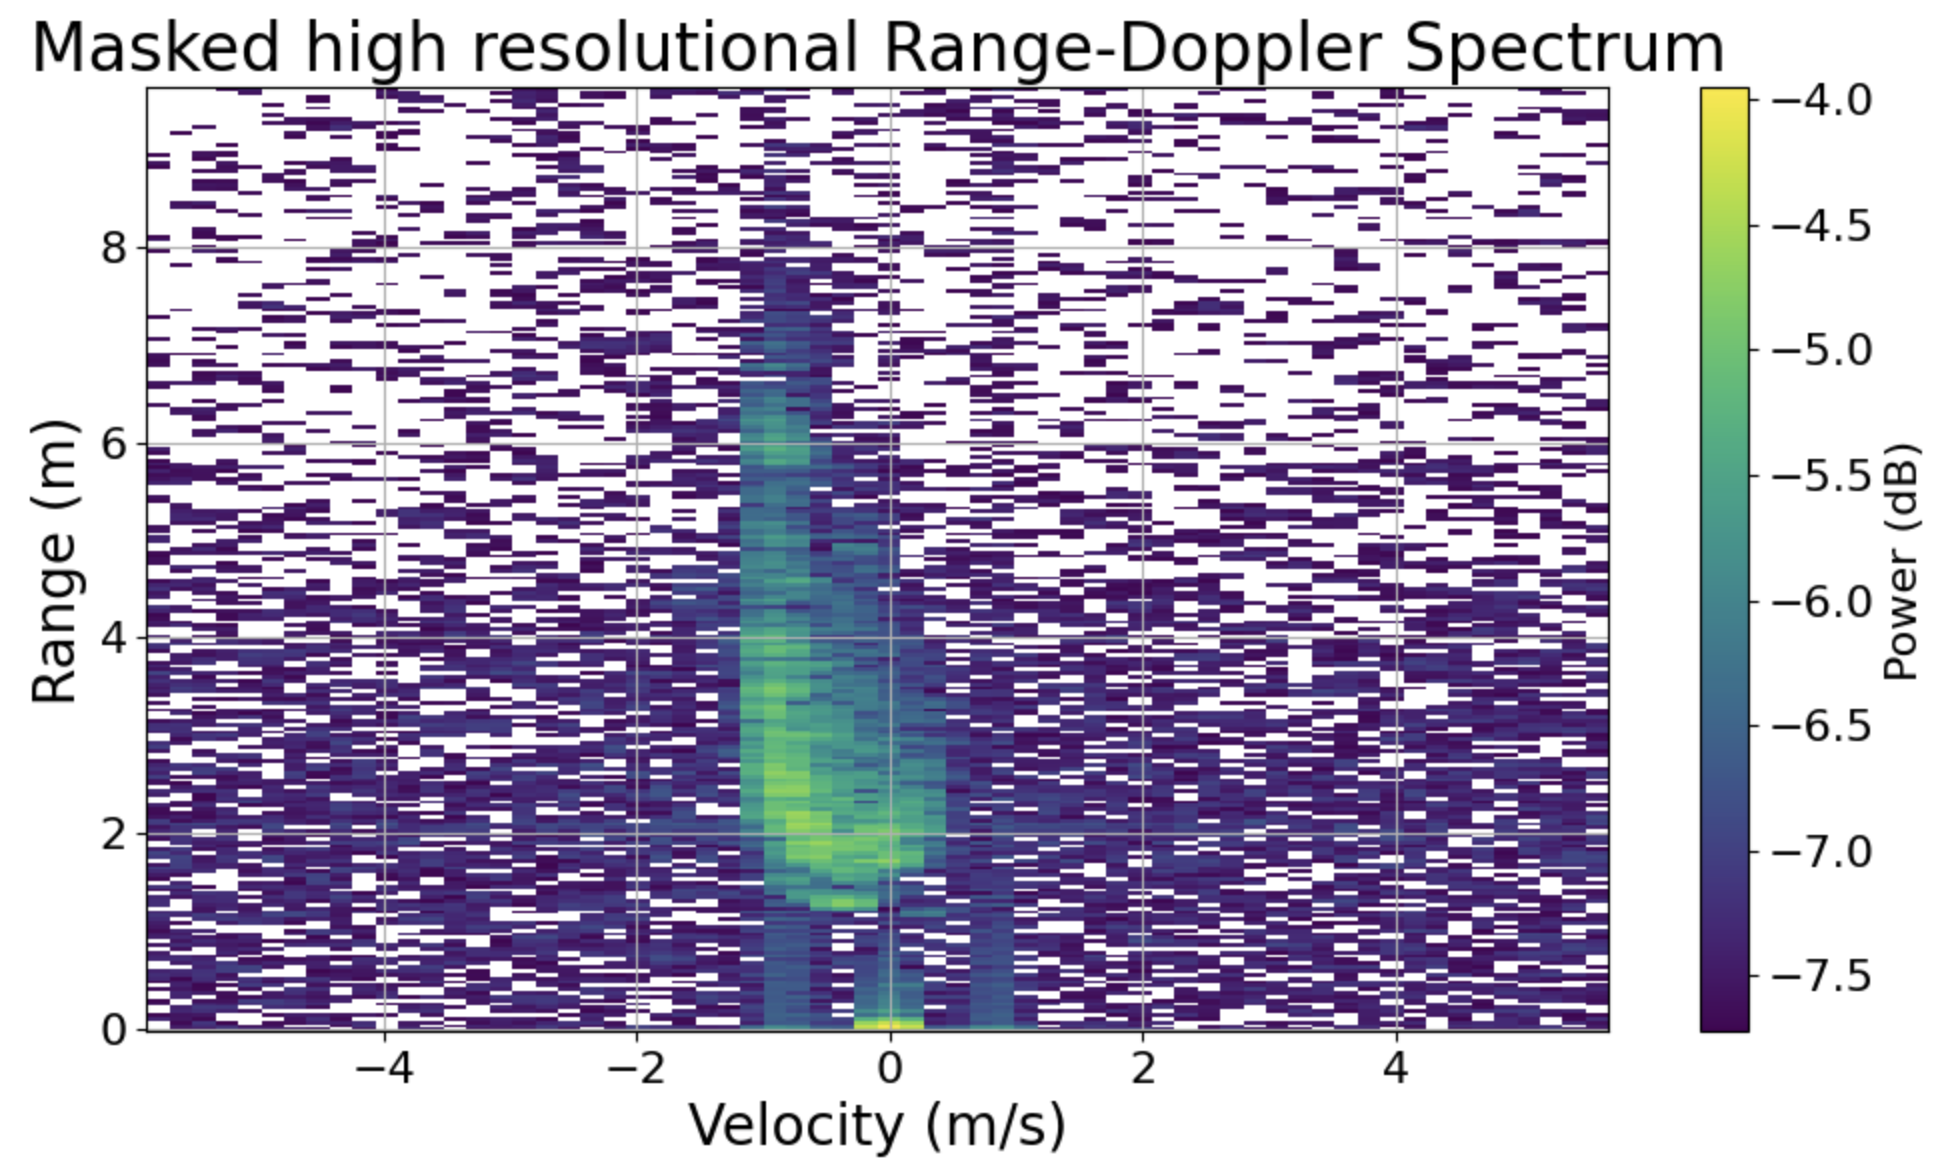
\includegraphics[scale=.24]{thesis/figures/masked_gt.png}}
        \caption{Masked high-resolution range-Doppler map}
        \label{masked high resolution image with logarithic amplitude}
    \end{subfigure}
    \caption{The mask operation on the high-resolution range-Doppler map with logarithic amplitude}
    \label{mask operation on the high resolution image with logarithic amplitude}
\end{figure}

In terms of the phase loss, the \gls{mse} can be used and combined with the scaling factor $\lambda$, namely
\begin{equation}
    \centering
    \mathcal{L}_{\text{LSD}} = \mathcal{L}_{\text{LSD, Amp}} + \lambda \times \mathcal{L}_{\text{MSE, Ph}},
\end{equation}

whereas in the evaluation phase, the scaling factor is set as zero, that is, only the amplitude \gls{lsd} loss is taken into consideration and the mask will not be used. Note that, if in the processing methods the logarithm is performed, both \gls{mse} and \gls{lsd} will have logarithmic operation on the amplitude, then the difference is only the square root in \gls{lsd} loss function. Conversely, if no logarithm operation in the processing methods, the \gls{lsd} loss function keeps using logarithm on the amplitude while the \gls{mse} doesn't have.

\subsection{PLSD}
Compared with the \gls{lsd} loss function, the difference of the \gls{plsd} loss function is that it doesn't use the \gls{mse} phase loss, that is,
\begin{equation}
    \centering
    \mathcal{L}_{\text{PLSD}} = \left\langle \left| \log_{10} \left| \frac{\hat{Y}}{Y} \right| \right| \times \left( 2 - \mathcal{R} \left\{ \frac{\hat{Y}}{Y} \right\} \right) \right\rangle,
\end{equation}

where
\begin{equation}
    \centering
    \mathcal{R} \left\{ \frac{\hat{Y}}{Y} \right\} = \cos{(\varphi_{\hat{Y}} - \varphi_{Y})}.
\end{equation}

\gls{plsd} loss function can be only used in training and validation phases if not amplitude representation type.

\section{Perceptual loss} \label{perceptual loss}
% show the different VGG layer
The \gls{vgg} \cite{simonyan_very_2015} are common models for image reconstruction, which is implemented using multiple blocks of the convolutional layers. Simonyan et al. proposed six \gls{vgg} configurations in different scales, each with the different number of layers and parameters, as shown in Table \ref{vgg configurations}, where the configuration E represents VGG19, which has the most parameters and the highest accuracy.

\begin{table}[t]
    \centering
    \caption{VGG configurations \cite{simonyan_very_2015}}
    \label{vgg configurations}
    % \renewcommand{\arraystretch}{1.3}
    \resizebox{0.99\textwidth}{!}{
    \begin{tabular}{|c|c|c|c|c|c|}
        \hline
        \multicolumn{6}{|c|}{\textbf{VGG Configuration}} \\ 
        \hline
        A & A-LRN & B & C & D & E \\ 
        \hline
        11 weight layers & 11 weight layers & 13 weight layers & 16 weight layers & 16 weight layers & 19 weight layers \\ 
        \hline
        \multicolumn{6}{|c|}{input (224 × 224 RGB image)} \\ 
        \hline
        conv3-64 & conv3-64 & conv3-64 & conv3-64 & conv3-64 & conv3-64 \\ 
          & \textbf{LRN} & \textbf{conv3-64} & conv3-64 & conv3-64 & conv3-64 \\ 
        \hline
        \multicolumn{6}{|c|}{maxpool} \\ 
        \hline
        conv3-128 & conv3-128 & conv3-128 & conv3-128 & conv3-128 & conv3-128 \\ 
          &   & \textbf{conv3-128} & conv3-128 & conv3-128 & conv3-128 \\ 
        \hline
        \multicolumn{6}{|c|}{maxpool} \\ 
        \hline
        conv3-256 & conv3-256 & conv3-256 & conv3-256 & conv3-256 & conv3-256 \\ 
        conv3-256 & conv3-256 & conv3-256 & conv3-256 & conv3-256 & conv3-256 \\ 
          &   &   & \textbf{conv1-256} & \textbf{conv3-256} & conv3-256 \\ 
          &   &   &   &   & \textbf{conv3-256} \\ 
        \hline
        \multicolumn{6}{|c|}{maxpool} \\ 
        \hline
        conv3-512 & conv3-512 & conv3-512 & conv3-512 & conv3-512 & conv3-512 \\ 
        conv3-512 & conv3-512 & conv3-512 & conv3-512 & conv3-512 & conv3-512 \\
          &   &   & \textbf{conv1-512} & \textbf{conv3-512} & conv3-512 \\
          &   &   &   &   & \textbf{conv3-512} \\
        \hline
        \multicolumn{6}{|c|}{maxpool} \\ 
        \hline
        conv3-512 & conv3-512 & conv3-512 & conv3-512 & conv3-512 & conv3-512 \\ 
        conv3-512 & conv3-512 & conv3-512 & conv3-512 & conv3-512 & conv3-512 \\
          &   &   & \textbf{conv1-512} & \textbf{conv3-512} & conv3-512 \\
          &   &   &   &   & \textbf{conv3-512} \\
        \hline
        \multicolumn{6}{|c|}{maxpool} \\ 
        \hline
        \multicolumn{6}{|c|}{FC-4096} \\  
        \hline
        \multicolumn{6}{|c|}{FC-4096} \\ 
        \hline
        \multicolumn{6}{|c|}{FC-1000} \\ 
        \hline
        \multicolumn{6}{|c|}{soft-max} \\ 
        \hline
    \end{tabular}
    }
\end{table}

Johnson et al. proposed a perceptual loss function based on the \gls{vgg} model, using the features extracted from different layers of the VGG model to calculate the loss between super-resolution and high-resolution data \cite{johnson_perceptual_2016}. Compared with the per-pixel loss function mentioned above, perceptual loss function can produce a more visually pleasing range-Doppler map. They proposed two types of the perceptual loss functions, one is about the feature reconstruction loss which is the Euclidean distance between the feature representation
\begin{equation}
    \centering
    \mathcal{L}_{\text{Perceptual}} (\hat{Y}, Y) = \frac{1}{H W C} \left\| \phi (\hat{Y}) - \phi (Y) \right\|_2^2,
\end{equation}

where $\phi(\cdot)$ denotes the feature extraction of the \gls{vgg} model and another type is based on the style of the image, namely
\begin{equation}
    \centering
    G^{\phi}(x)_{c, c'} = \frac{1}{H W C} \sum_{h=1}^{H} \sum_{w=1}^{W} \phi (\hat{Y})_{h,w,c} \phi (Y)_{h,w,c'}.
\end{equation}

In our case, the upsampling data is specifically the range-Doppler map, therefore, the feature reconstruction perceptual loss is used rather than the style. In \gls{vgg} model, with the deeper channel of blocks, the representation of each block changes. In the first two blocks, the shallow features are learned, such as margin, color and brightness. Since the third block, more deeper feature are represented, such as texture. And in fourth and fifth blocks, some distinguished features are extracted. Therefore, in the perceptual loss function of the pipeline, the last layer of the first four blocks in the pretrained \gls{vgg} model provided by TensorFlow are used to extract the feature representation by default, since it can mitigate the loss computation to be much expensive. Furthermore, since the channel dimension of the range-Doppler map is just one, while in the \gls{vgg} model, RGB image is used for pretraining, the range-Doppler map has to extend the channel dimension.

\section{Combination of the losses} \label{combination of the losses}
% combination of the loss functions such as LSD+Perceptual loss functions, as well as the pre-training with the single loss function firstly while combination.
According to the various loss functions mentioned above, their types and goals are somewhat different. For example, \gls{lsd} loss function uses logarithmic operations to pay more attention on the signal with low amplitude, while the perceptual loss function improves the overall perception of the range-Doppler map using the feature representation. Therefore, different types of loss functions can be combined with each other, such as
\begin{equation}
    \centering
    \mathcal{L}_{\text{Combination}} = \mathcal{L}_{\text{LSD}} + \lambda_c \times \mathcal{L}_{\text{Perceptual}},
    \label{loss combination equation}
\end{equation}

where $\lambda_c$ as a hyperparameter that can be tuned according to the importance or the values of both loss functions. Moreover, in order to improve the stability, the pretraining operation can be used, that is, the model can be trained with one loss of the loss combination and after a few epochs trained by both. Otherwise, at the very beginning of the training, if the perceptual loss is relatively large, it would cause too much attention on the perception rather than the target \gls{lsd} loss per pixels.

\section{Adversarial loss} \label{gan loss}
% show both generator loss and discriminator loss
In \gls{cgan} model, the generator and discriminator models will be trained mutually, whereas the loss functions for both are different. Therefore in this section, the generator loss function and discriminator loss function will be shown respectively.

\subsection{Generator loss}
For the generator model, on one hand, it should reduce the value of the loss combination, such as the \gls{lsd} combining with perceptual loss, after multiple epochs of training, and on the other hand, it should make the discriminator believe that the super-resolution range-Doppler map is the real high-resolution range-Doppler map. Since the output of the discriminator model is a probability value, the adversarial loss for the generator part should be regarded as the difference between this probability and 100\%, that is,
\begin{equation}
    \centering
    \mathcal{L}_{\text{GAN, Gen}} = \| 1 - P_{\text{Super}} \|_{2},
\end{equation}

where $P_{\text{Super}}$ represents the probability value of the super-resolution range-Doppler map as the real high-resolution range-Doppler map from the discriminator model. The total generator loss function should combine with the target loss function mentioned above, namely
\begin{equation}
    \centering
    \mathcal{L}_{\text{Gen}} = \mathcal{L}_{\text{Combination}} + \lambda_g \times \mathcal{L}_{\text{GAN, Gen}},
\end{equation}

\subsection{Discriminator loss}
For the discriminator model, its goal is to make the probability of identifying the super-resolution and ground truth as real high-resolution range-Doppler maps approaching 0 and 1 respectively. Therefore, the discriminator loss function also contains two parts, namely
\begin{equation}
    \centering
    \mathcal{L}_{\text{Disc}} = \| 1 - P_{\text{High}} \|_{2} + \| 0 - P_{\text{Super}} \|_{2},
\end{equation}

where $P_{\text{High}}$ is the probability value that the ground truth is really the high-resolution range-Doppler map.
